%%%%%%%%%%%%%%%%%%%%%%%%%%%%%%%%%%%%%%%%%%%%%%%%%%%%%%%%%%%%%%%%%%%%%%%%%%%%%%%
%
% \chapter{Finite element formulations}\label{chFEMForms}
%
%%%%%%%%%%%%%%%%%%%%%%%%%%%%%%%%%%%%%%%%%%%%%%%%%%%%%%%%%%%%%%%%%%%%%%%%%%%%%%%%

ERMES 20.0 solves numerically the time-harmonic Maxwell's equations with the Finite Element Method (FEM). This appendix presents the FEM approaches implemented in ERMES 20.0 along with its advantages and disadvantages. The FEM formulations implemented in ERMES 20.0 are: 
\begin{itemize}
	\itemsep0em 
	\item Double-curl Maxwell's equations with edge elements,
	\item Regularized Maxwell's equations with nodal elements,
	\item Local $L^{2}$ projection method with nodal and bubble elements.
\end{itemize}
All the above formulations include an $\textbf{A}-\phi$ potentials version and switchable stabilization terms with Lagrange multipliers. All the possible combinations that can be used in ERMES 20.0 (formulation type, \textbf{E} field or $\textbf{A}-\phi$ potentials, stabilization on/off) will be presented in the following. This appendix assumes a reader with knowledge on FEM. Therefore, the weak form of each formulation will be introduced without justification. For more details on FEM fundamentals, we recommend the references \cite{Jin, Monk, LuisGarcia, Ferrari, Johnson, Zienkiewicz}.

\section{Introduction}\label{FEMIntro}

The typical approach when solving a general electromagnetic problem with FEM is to use edge elements with the double-curl Maxwell's equations. The edge elements proposed by N\'{e}d\'{e}lec \cite{Nedelec} seem to be the answer to most of the drawbacks exhibited by FEM when applied to electromagnetism \cite{Jin, LuisGarcia}. With edge elements, spurious-free solutions are obtained, boundary conditions are easier to implement and, the normal discontinuity and tangential continuity between different media are automatically satisfied. In addition, they present a better behaviour in non-convex domains than Lagrangian elements \cite{EdgeElementsPuntiagudo}. However, using the double-curl with edge elements formulation has also disadvantages \cite{EdgeElementsFallacy, EdgeElementsProsNo}. The most important one being the ill-conditioning of the generated matrices, which can even be singular in problems with a high number of unknowns \cite{SingularEE}. The use of stabilization methods with Lagrange multipliers are reported to improve the conditioning of the matrix in \cite{AugmentedFormulations, HiptmairReport}, or even be necessary to reach convergence \cite{Kikuchi, Ledger-hp}, but at the cost of increasing the number of unknowns. In our experience with ERMES, adding extra stabilization terms did not improve visibly the conditioning of the matrices nor the slow convergence of iterative solvers. The inclusion of Lagrange multipliers only showed to be useful at low frequencies, when they were practically mandatory for solving with direct methods. Therefore, although edge elements present several advantageous features, its FEM linear systems can be computationally expensive and difficult to solve. Because of this, it would be desirable to explore other FEM approaches that, maybe, will be able to provide better conditioned matrices.

An alternative approach to improve the FEM matrix conditioning problem is based on nodal elements and the regularized Maxwell's equations \cite{BC-OJOOut, WeightedRegularizedME}. The main advantages of this alternative formulation are that it provides spurious-free solutions with well-conditioned matrices and, moreover, only the three components of \textbf{E} are the unknowns; that is, there is no need of extra terms with Lagrange multipliers for stabilization purposes. Furthermore, its integral representation involves a less singular kernel (order 1 instead of 3), which makes the regularized FEM formulation best suited to hybridization with integral numerical techniques \cite{BC-OJOOut}. A study demonstrating the better computational performance of the nodal regularized formulation when compared with the edge elements double-curl approach was done in \cite{WRME-Performance}. Unfortunately, new difficulties arise that were not present in the previous approach. The main drawback is that a non-physical solution can be obtained when the electromagnetic field has a singularity in the problem domain. Also, boundary conditions and field discontinuities are more laborious to implement. In this appendix is shown how ERMES 20.0 overcomes these difficulties.

The third FEM approach implemented in ERMES 20.0 is based on the Local $L^{2}$ Projection (LL2P) method and it uses nodal and bubble elements \cite{L2P-BE, L2P-BE-P}. The LL2P method main advantages are that it solves the singularity problem that affects the regularized formulation while still producing well-conditioned FEM matrices. Moreover, it does not need extra terms with Lagrange multipliers for stabilization purposes. Unfortunately, this approach is the most computationally demanding of the three presented here because of the bubble elements required for its stabilization. Anyway, the LL2P formulation can be useful on some scenarios where the other two methods can struggle to reach a solution. 

\section{Double-curl Maxwell's equations with edge elements}\label{DoubleCurlEdge}

The generic problem to solve consists in finding the electric field \textbf{E} in a domain $\Omega$ with boundary $\partial\Omega$ produced by a current source \textbf{J} oscillating at an angular frequency $\omega$. The equation that \textbf{E} satisfies in $\Omega$ is the so-called \emph{double-curl Maxwell's equation} (see Section \ref{sWaveEquation}):
\begin{equation}\label{CurlCurlME}
	\nabla\times\left(\frac{1}{\mu}\nabla\times\mathbf{E}\right) - \omega^{2}\varepsilon\mathbf{E} = i\omega\mathbf{J},
\end{equation}
where $\mu$ and $\varepsilon$ are, respectively, the complex magnetic permeability and the complex electric permittivity. If $\Omega$ is filled with Isotropic Homogeneous Linear (IHL) materials then, the definitions of $\mu$ and $\varepsilon$ are given in Section \ref{MaxwellFD-LIM}. If $\Omega$ contains a cold plasma then, $\varepsilon$ is the cold plasma tensor derived in \cite{Swanson, Stix}. 

Equation \ref{CurlCurlME} must be supplemented with information about the behaviour of the fields on the boundary $\partial\Omega$ to have a unique solution in $\Omega$. On the surface of a Perfect Electric Conductor (PEC), the field \textbf{E} satisfies the following boundary condition (see Section \ref{sPECcond}):
\begin{equation}\label{BC-PEC}
	\mathbf{\hat{n}}\times\mathbf{E} = 0.
\end{equation}
On the surface of a Perfect Magnetic Conductor (PMC), or symmetry surface, the field \textbf{E} satisfies:
\begin{equation}\label{BC-PMC}
	\mathbf{\hat{n}}\times\nabla\times\mathbf{E} = 0.
\end{equation}
In an open domain, the Silver-M\"{u}ller radiation boundary condition must be added at infinity (see Section \ref{sSMradcond}):
\begin{equation}\label{RadiationBoundaryCondition}
	\lim_{r\rightarrow\infty}\oint_{\partial\Omega_{r}}\|\,\mathbf{\hat{n}}\times\nabla\times\mathbf{E}\, +\,(i\omega\sqrt{\epsilon_{0}\mu_{0}})\,\mathbf{E}\,\|^{2} = 0.
\end{equation}
In a waveguide port, the boundary conditions must account for the specific propagative modes of the waveguide. For instance, in a rectangular waveguide port, with only the fundamental mode $\text{TE}_{10}$ propagating, the boundary condition can be expressed as:
\begin{equation}\label{BC-WBC}
	\mathbf{\hat{n}}\times\nabla\times\mathbf{E} = \gamma\,(\mathbf{\hat{n}}\times\mathbf{\hat{n}}\times\mathbf{E}) + \mathbf{U},
\end{equation}
where $\gamma$ is the propagation constant of the fundamental mode, and
\begin{equation}\label{WGPortConditionsU}
	\begin{aligned}
		\mathbf{U} &= -2\,\gamma\,(\mathbf{\hat{n}}\times\mathbf{\hat{n}}\times\mathbf{E}_{10}),
		\\
		\mathbf{U} &= 0
	\end{aligned}
\end{equation}
for the input and the output port, respectively \cite{Jin}. The field $\mathbf{E}_{10}$ is the incident mode $\text{TE}_{10}$ imposed at the input port. Boundary condition \eqref{BC-WBC} can be adapted to represent the behaviour of \textbf{E} on the surface of an imperfect conductor (see Section \ref{sIBCcond}), or to approximate the Silver-M\"{u}ller radiation boundary condition \eqref{RadiationBoundaryCondition} with the so-called \textit{first order Absorbing Boundary Condition} (1st ABC):
\begin{equation}\label{BC-1stABC}
	\mathbf{\hat{n}}\times\nabla\times\mathbf{E} = i\omega\sqrt{\epsilon_{0}\mu_{0}}\, (\mathbf{\hat{n}}\times\mathbf{\hat{n}}\times\mathbf{E}).
\end{equation}
The above set of equations is solved in ERMES 20.0 using an equivalent weak formulation, that is, if $L^{2}(\Omega)$ is the Hilbert space of all the square-integrable functions in $\Omega$ and $\mathbf{H}_{0}(\mathbf{curl};\Omega)$ is defined as
\begin{equation}\label{HCurl}
	\mathbf{H}_{0}(\mathbf{curl};\Omega) := \{\,\mathbf{F}\in \mathbf{L}^{2}(\Omega)\enspace|\enspace\nabla\times \mathbf{F} \in \mathbf{L}^{2}(\Omega),\enspace \mathbf{\hat{n}}\times\mathbf{F} = 0\enspace\text{in PEC}\,\}
\end{equation}
then, solving equation \eqref{CurlCurlME} is equivalent to find an $\mathbf{E} \in \mathbf{H}_{0}(\mathbf{curl};\Omega)$ such
that $\forall\,\mathbf{F} \in \mathbf{H}_{0}(\mathbf{curl};\Omega)$ holds:
\begin{equation}\label{CurlCurlWeak}
	\int_{\Omega}\enspace\frac{1}{\mu}(\nabla\times\mathbf{E})\cdot(\nabla\times\mathbf{\bar{F}})\, - \,\omega^{2}\int_{\Omega}\varepsilon\mathbf{E}\cdot\mathbf{\bar{F}}\, + \,\textbf{B.C.}|_{\partial\Omega}\, = \,i\omega\int_{\Omega}\mathbf{J}\cdot\mathbf{\bar{F}},
\end{equation}
where the bar over the magnitudes denotes its complex conjugate and $\textbf{B.C.}|_{\partial\Omega}$ is the term that accounts for the boundary conditions:
\begin{equation}\label{BCGeneral-WF}
	\textbf{B.C.}|_{\partial\Omega}\enspace = \enspace\int_{\partial\Omega}\enspace\frac{1}{\mu}\left(\mathbf{\hat{n}}\times\nabla\times\mathbf{E}\right)\cdot\mathbf{\bar{F}}.
\end{equation}
The weak formulation \eqref{CurlCurlWeak} discretized with edge elements is the classical way to apply FEM to electromagnetic field problems. In ERMES 20.0, the weak formulation \ref{CurlCurlWeak} is available with the first and second order edge elements given in references \cite{Jin, LuisGarcia}. The advantages and disadvantages of this approach were cited at the introduction of this appendix. 

\subsection{$\textbf{A}-\phi$ potentials}\label{sEdgePotentials}

ERMES 20.0 has available an $\textbf{A}-\phi$ potentials version of the double-curl formulation. The $\textbf{A}-\phi$ version can be useful at low frequencies where the \textbf{E} field version can be numerically unstable and difficult to solve. The $\textbf{A}-\phi$ version uses the potentials defined in Section \ref{sAVPotentials} adapted to frequency domain as discussed in \ref{sEMTH}:
\begin{eqnarray}\label{DefPotentialsFD} 
	\mathbf{B} &=& \nabla\times\mathbf{A}, 
	\label{DefBPotentialsFD}
	\\
	\mathbf{E} &=& i\omega\mathbf{A} - \nabla\phi.
	\label{DefEPotentialsFD}
\end{eqnarray}
The set of differentials equations that these time-harmonic potentials must satisfy is:
\begin{equation}\label{CCAVDE}
	\begin{aligned}
		\nabla\times\left(\frac{1}{\mu}\nabla\times\mathbf{A}\right) - \omega^{2}\varepsilon\left(\mathbf{A} + \nabla\phi^{'}\right) &= \mathbf{J},
		\\
		\nabla\left(\omega^{2}\varepsilon\left(\mathbf{A} + \nabla\phi^{'}\right)\right) &= 0,
	\end{aligned}
\end{equation}
where the scalar potential $\phi$ has been substituted by $\phi^{'}$ to guarantee the symmetry of the FEM matrix, being $\phi^{'}$ defined as:
\begin{equation}\label{PhiReDef}
	\phi = -i\omega\phi^{'}.
\end{equation}
On the surface of a perfect electric conductor, $\textbf{A}$ and $\phi^{'}$ must satisfy an equivalent boundary condition to the PEC condition given in \ref{BC-PEC}:
\begin{equation}\label{PEC-AV-CC}
	\begin{aligned}
		\mathbf{\hat{n}}\times\mathbf{A} &= 0,
		\\
		\phi^{'} &= \phi^{'}_{0},
	\end{aligned}
\end{equation}
where $\phi_{0} = -i\omega\phi^{'}_{0}$ is a voltage imposed on the PEC surface. Similarly, on a PMC symmetry surface, $\textbf{A}$ and $\phi^{'}$ must satisfy:
\begin{equation}\label{PMC-AV-CC}
	\begin{aligned}
		\mathbf{\hat{n}}\times\nabla\times\mathbf{A} &= 0,
		\\
		\mathbf{\hat{n}}\cdot\left(\varepsilon\mathbf{A} + \varepsilon\nabla\phi^{'}\right) &= 0.
	\end{aligned}
\end{equation}
In a Robin boundary surface, where waveguide ports or radiation boundary conditions could be applied, the potentials must satisfy:
\begin{equation}\label{RBC-AV-CC}
	\begin{aligned}
		\mathbf{\hat{n}}\times\nabla\times\mathbf{A} - \gamma(\mathbf{\hat{n}}\times\mathbf{\hat{n}}\times\mathbf{A}) &= \mathbf{U}^{'},
		\\
		\mathbf{\hat{n}}\cdot\left(\varepsilon\mathbf{A} + \varepsilon\nabla\phi^{'}\right) &= \,0,
	\end{aligned}
\end{equation}
where $\mathbf{U}^{'} = \mathbf{U}/i\omega$, and $\gamma$ and $\mathbf{U}$ are the same as those defined in \ref{BC-WBC}-\ref{WGPortConditionsU}. The set of equations \ref{CCAVDE} plus the boundary conditions \ref{PEC-AV-CC}-\ref{RBC-AV-CC} are solved in ERMES 20.0 using the following weak formulation; if $H_{0}(grad;\Omega)$ is the functional space defined as:
\begin{equation}\label{HGrad}
	H_{0}(grad;\Omega) := \{\,G\in L^{2}(\Omega)\enspace|\enspace\nabla G \in L^{2}(\Omega),\enspace G = G_{0}\enspace\text{in PEC}\,\}
\end{equation}
then, solving the system \ref{CCAVDE}-\ref{RBC-AV-CC} is equivalent to find an $\mathbf{A} \in \mathbf{H}_{0}(\mathbf{curl};\Omega)$ and $\phi^{'} \in H_{0}(grad;\Omega)$ such
that $\forall\,\mathbf{F} \in \mathbf{H}_{0}(\mathbf{curl};\Omega)$ and $\forall\,G \in H_{0}(grad;\Omega)$ holds:
\begin{equation}\label{CurlCurlWeakAV}
    \begin{aligned}
	\int_{\Omega}\enspace\frac{1}{\mu}(\nabla\times\mathbf{A})\cdot(\nabla\times\mathbf{\bar{F}})\, - \,\omega^{2}\int_{\Omega}\varepsilon\left(\mathbf{A} + \nabla\phi^{'}\right)\cdot\mathbf{\bar{F}}\, + \,\textbf{P.B.C.}|_{\partial\Omega}\, &= \int_{\Omega}\mathbf{J}\cdot\mathbf{\bar{F}},
	\\
	-\,\omega^{2}\int_{\Omega}\varepsilon\left(\mathbf{A} + \nabla\phi^{'}\right)\cdot\nabla\bar{G}\, + \,\omega^{2}\int_{\partial\Omega}\mathbf{\hat{n}}\cdot\left(\varepsilon\mathbf{A} + \varepsilon\nabla\phi^{'}\right)\bar{G}\, &= 0	
    \end{aligned}
\end{equation}
where $\textbf{P.B.C.}|_{\partial\Omega}$ accounts for the boundary conditions and it is equivalent to the term $\textbf{B.C.}|_{\partial\Omega}$ defined in \ref{BCGeneral-WF}:
\begin{equation}\label{BCGeneral-CCAV}
	\textbf{P.B.C.}|_{\partial\Omega}\enspace = \enspace\int_{\partial\Omega}\enspace\frac{1}{\mu}\left(\mathbf{\hat{n}}\times\nabla\times\mathbf{A}\right)\cdot\mathbf{\bar{F}}.
\end{equation}
In ERMES 20.0, the weak formulation \ref{CurlCurlWeakAV} has been implemented with first and second order edge elements for \textbf{A} and first order nodal elements for $\phi^{'}$. 

\subsection{Stabilization}\label{EdgeDoubleCurlStab}

Formulations \ref{CurlCurlWeak} and \ref{CurlCurlWeakAV} may require the presence of extra stabilization terms at low frequencies, when the solution is near the degenerate kernel of the double-curl operator. This extra stabilization can be achieved by controlling the divergence with Lagrange multipliers. ERMES 20.0 implements one of the several possible strategies proposed in \cite{Monk}. Following this strategy, formulation \ref{CurlCurlWeak} can be re-expressed as; find $\mathbf{E} \in \mathbf{H}_{0}(\mathbf{curl};\Omega)$ and $\varphi \in H_{0}(grad;\Omega)$ such as $\forall\,\mathbf{F} \in \mathbf{H}_{0}(\mathbf{curl};\Omega)$ and $\forall\,\xi \in H_{0}(grad;\Omega)$ holds:
\begin{equation}\label{CurlCurlWeakS}
    \begin{aligned}
	    \int_{\Omega}\frac{1}{\mu}(\nabla\times\mathbf{E})\cdot(\nabla\times\mathbf{\bar{F}}) - \omega^{2}\int_{\Omega}\varepsilon\mathbf{E}\cdot\mathbf{\bar{F}} + \int_{\Omega}\varepsilon\mathbf{F}\cdot\nabla\varphi + \textbf{B.C.}|_{\partial\Omega} &= i\omega\int_{\Omega}\mathbf{J}\cdot\mathbf{\bar{F}},
	    \\
	    \int_{\Omega}\varepsilon\mathbf{E}\cdot\nabla\xi - \int_{\Omega}\varepsilon\nabla\varphi\cdot\nabla\xi &= 0.
    \end{aligned}
\end{equation}
Similarly, the potential formulation \ref{CurlCurlWeakAV} is stabilized in ERMES 20.0 using the following weak form; find $\mathbf{A} \in \mathbf{H}_{0}(\mathbf{curl};\Omega)$, $\phi^{'} \in H_{0}(grad;\Omega)$ and, $\varphi \in H_{0}(grad;\Omega)$ such
that $\forall\,\mathbf{F} \in \mathbf{H}_{0}(\mathbf{curl};\Omega)$, $\forall\,G \in H_{0}(grad;\Omega)$ and, $\forall\,\xi \in H_{0}(grad;\Omega)$ holds:
\begin{equation}\label{CurlCurlWeakAVS2}
	\nonumber
	\begin{aligned}
	    \int_{\Omega}\frac{1}{\mu}(\nabla\times\mathbf{A})\cdot(\nabla\times\mathbf{\bar{F}}) - \omega^{2}\int_{\Omega}\varepsilon\left(\mathbf{A} + \nabla\phi^{'}\right)\cdot\mathbf{\bar{F}} + \int_{\Omega}\mathbf{F}\cdot\nabla\varphi + \textbf{P.B.C.}|_{\partial\Omega} &= \int_{\Omega}\mathbf{J}\cdot\mathbf{\bar{F}},
        \\
        -\,\omega^{2}\int_{\Omega}\varepsilon\left(\mathbf{A} + \nabla\phi^{'}\right)\cdot\nabla\bar{G}\, + \,\omega^{2}\int_{\partial\Omega}\mathbf{\hat{n}}\cdot\left(\varepsilon\mathbf{A} + \varepsilon\nabla\phi^{'}\right)\bar{G}\, &= 0,	
        \\
        \int_{\Omega}\mathbf{A}\cdot\nabla\xi - \int_{\Omega}\nabla\varphi\cdot\nabla\xi &= 0.	
	\end{aligned}
\end{equation}
In ERMES 20.0, the above stabilized formulations has been implemented with first and second order edge elements for \textbf{E} and \textbf{A}, and first order nodal elements for $\phi^{'}$ and $\varphi$.

\section{Regularized Maxwell's equations with nodal elements}\label{RMENodal}

An equivalent approach for solving \eqref{CurlCurlME} is to use the so-called \emph{regularized Maxwell's equation}:
\begin{equation}\label{RegularizedME}
	\nabla\times\left(\frac{1}{\mu}\nabla\times\mathbf{E}\right) - \bar{\varepsilon}\,\nabla\left(\frac{1}{\tau\mu}\nabla\cdot(\varepsilon\mathbf{E})\right) - \omega^{2}\varepsilon\mathbf{E} = i\omega\mathbf{J},
\end{equation}
were $\varepsilon$ represents a generic permittivity tensor and $\tau = tr(\bar{\varepsilon}\varepsilon)/3$. In the case of IHL materials, $\tau$ can be simplified to $\tau = \| \varepsilon \|^{2}$. Equation \ref{RegularizedME} must also be supplemented with boundary conditions on $\partial\Omega$ to guarantee a unique solution in $\Omega$. These boundary conditions need to be adapted to the new regularized approach. For instance, on the surface of a perfect electric conductor, the regularized version of the PEC boundary condition \eqref{BC-PEC} is:
\begin{equation}\label{BC-RPEC}
	\begin{aligned}
		\nabla\cdot(\varepsilon\mathbf{E}) &= 0,
		\\
		\mathbf{\hat{n}}\times\mathbf{E} &= 0.
	\end{aligned}
\end{equation}
On the surface of a perfect magnetic conductor, the regularized version of the PMC boundary condition \eqref{BC-PMC} is:
\begin{equation}\label{BC-RPMC}
	\begin{aligned}
		\mathbf{\hat{n}}\times\nabla\times\mathbf{E} &= 0,
		\\
		\mathbf{\hat{n}}\cdot\mathbf{E} &= 0.
	\end{aligned}
\end{equation}
On an infinite open domain, the regularized version of the Silver-M\"{u}ller radiation boundary condition \eqref{RadiationBoundaryCondition} is: 
\begin{equation}\label{SilverMullerExtend}
	\begin{aligned}
		\lim_{r\rightarrow\infty}&\oint_{\partial\Omega_{r}}\|\,\mathbf{\hat{n}}\times\nabla\times\mathbf{E}\,-\,i\omega\sqrt{\epsilon_{0}\mu_{0}} \, (\mathbf{\hat{n}}\times\mathbf{\hat{n}}\times\mathbf{E})\,\|^{2} =
		0,
		\\
		&\enspace\enspace\lim_{r\rightarrow\infty}\oint_{\partial\Omega_{r}}|\,\nabla\cdot\mathbf{E}\,-\,i\omega\sqrt{\epsilon_{0}\mu_{0}} \, (\mathbf{\hat{n}}\cdot\mathbf{E})\,|^{2} = 0,
	\end{aligned}
\end{equation}
and its regularized 1st ABC approximation:
\begin{equation}\label{ABCExtend}
	\begin{aligned}
		\mathbf{\hat{n}}\times\nabla\times\mathbf{E} &= i\omega\sqrt{\epsilon_{0}\mu_{0}}\left(\mathbf{\hat{n}}\times\mathbf{\hat{n}}\times\mathbf{E}\right),
		\\
		\nabla\cdot\mathbf{E} &= i\omega\sqrt{\epsilon_{0}\mu_{0}}\left(\mathbf{\hat{n}}\cdot\mathbf{E}\right).
	\end{aligned}
\end{equation}
On waveguide ports, boundary condition \eqref{BC-WBC} must be adapted to the regularization as:
\begin{equation}\label{BC-RWPC}
	\begin{aligned}
		\mathbf{\hat{n}}\times\nabla\times\mathbf{E} &= \gamma\,(\mathbf{\hat{n}}\times\mathbf{\hat{n}}\times\mathbf{E}) + \mathbf{U},
		\\
		\nabla\cdot\mathbf{E} &= \gamma\,\left(\mathbf{\hat{n}}\cdot\mathbf{E}\right).
	\end{aligned}
\end{equation}
The above set of equations is solved in ERMES 20.0 using an equivalent regularized weak formulation; that is, if $\mathbf{H}_{0}(\mathbf{curl},\text{div};\Omega)$ is the functional space defined as
\begin{equation}\label{HcurlDiv}
	\begin{aligned}
		\mathbf{H}_{0}(\mathbf{curl},\text{div};\Omega):=\{\,\mathbf{F}\in \mathbf{L}^{2}(\Omega)\,|\,\nabla&\times \mathbf{F}\in\mathbf{L}^{2}(\Omega),\,\nabla\cdot(\varepsilon\mathbf{F})\in L^{2}(\Omega),\\ \mathbf{\hat{n}}&\times\mathbf{F} = 0\enspace\text{in PEC},\,\mathbf{\hat{n}}\,\cdot\,\mathbf{F} = 0\enspace\text{in PMC}\,\},
	\end{aligned}
\end{equation}
solving \eqref{RegularizedME} is equivalent to find an $\,\,\mathbf{E}\,\in\,\mathbf{H}_{0}(\mathbf{curl},\text{div};\Omega)\,\,$
such that $\,\,\forall\,\mathbf{F}\,\in\,\mathbf{H}_{0}(\mathbf{curl},\text{div};\Omega)\,\,$, the following holds:
\begin{equation}\label{RegularizedWeak}
	\begin{aligned}
		\int_{\Omega}\enspace\frac{1}{\mu}\left(\nabla\times\mathbf{E}\right)\cdot\left(\nabla\times\mathbf{\bar{F}}\right)\, + \,\int_{\Omega}\enspace\frac{1}{\tau\mu}\left(\nabla\cdot\left(\varepsilon\mathbf{E}\right)\right)\left(\nabla\cdot\left(\bar{\varepsilon}\mathbf{\bar{F}}\right)\right)
		\\
		\,\,\,\,-\enspace\omega^{2}\int_{\Omega}\varepsilon\mathbf{E}\cdot\mathbf{\bar{F}}\enspace + \enspace \textbf{R.B.C.}|_{\partial\Omega}\enspace = \enspace i\omega\int_{\Omega}\mathbf{J}\cdot\mathbf{\bar{F}},
	\end{aligned}
\end{equation}
where $\textbf{R.B.C.}|_{\partial\Omega}$ is the term, properly adapted to the regularization, that accounts for the boundary conditions:
\begin{equation}\label{RBCGeneral-RWF}
	\textbf{R.B.C.}|_{\partial\Omega} = \int_{\partial\Omega}\enspace\frac{1}{\mu}\left(\mathbf{\hat{n}}\times\nabla\times\mathbf{E}\right)\cdot\mathbf{\bar{F}}\, - \,\int_{\partial\Omega}\enspace\frac{1}{\tau\mu}\left(\nabla\cdot\left(\varepsilon\mathbf{E}\right)\right)\left(\mathbf{\hat{n}}\cdot\left(\bar{\varepsilon}\mathbf{\bar{F}}\right)\right).
\end{equation}
The equivalence between the \emph{classical} problem \eqref{CurlCurlME}-\eqref{BCGeneral-WF} and the \emph{regularized} problem \eqref{RegularizedME}-\eqref{RBCGeneral-RWF} is formally demonstrated in \cite{BC-OJOOut}. Although equation \eqref{RegularizedWeak} looks like a penalized method, the regularized formulation has no undetermined constants and, with the help of the extra boundary condition terms, the problem is well-posed. It is worth emphasizing the importance of the extra boundary conditions: if they are omitted, the number of iterations needed for an iterative solver to converge can severely increase or even spurious solutions can appear. In ERMES 20.0 the regularized formulation is available for first and second order nodal (Lagrangian) elements.

As mentioned in the introduction of this appendix, the regularized approach has the main features sought in an efficient FEM formulation; that is, it calculates spurious-free solutions with \textbf{E} as the only unknown and, it produces well-conditioned matrices. Unfortunately, to avoid unphysical solutions, special care must be taken in the discontinuity surface between different media and in the presence of fields singularities. The following subsections explain how ERMES 20.0 solve these problems. 

\subsection{Field discontinuities}\label{Discontinuities}

The regularized formulation requires nodal elements because of the properties imposed to its FEM bases in \ref{HcurlDiv}-\ref{RegularizedWeak}. Nodal elements force normal and tangential continuity on its interfaces therefore, in the presence of a field discontinuity (see Section \ref{sEMInterface}), special techniques must be applied. ERMES 20.0 uses the method explained in \cite{DobleNodo} to deal with field discontinuities. This method consists of defining two different nodes (one on each side of the discontinuity) and, during the assembly procedure, relate the two nodes as follows:
\begin{equation}\label{DobleNodeMatrix}
	\begin{aligned}
		\left(\begin{array}{c}
			E_{x}^{+}\\
			E_{y}^{+}\\
			E_{z}^{+}
		\end{array}\right) =
		\left(\begin{array}{lll}
			n_{x}^{2}\xi+1            & n_{x}^{2}n_{y}^{2}\xi     & n_{x}^{2}n_{z}^{2}\xi  \\
			n_{x}^{2}n_{y}^{2}\xi     & n_{y}^{2}\xi+1            & n_{y}^{2}n_{z}^{2}\xi  \\
			n_{x}^{2}n_{z}^{2}\xi     & n_{y}^{2}n_{z}^{2}\xi     &
			n_{z}^{2}\xi+1
		\end{array}\right)
		\left(\begin{array}{c}
			E_{x}^{-}\\
			E_{y}^{-}\\
			E_{z}^{-}
		\end{array}\right)
	\end{aligned}
\end{equation}
being
\[
\xi = \frac{\epsilon^{-} + i\left(\sigma^{-}/\omega\right)}{\epsilon^{+} + i\left(\sigma^{+}/\omega\right)} - 1,
\]
$\mathbf{n} = (n_{x},n_{y},n_{z})$ is the unit normal at the surface, and superscripts "+" and "-" denote each side of the discontinuity surface. In this method, the node on side "+" is removed from the global linear system with the help of \eqref{DobleNodeMatrix}, and only the unknowns on the side "-" are solved. No extra unknowns are added, and the symmetry of the total FEM matrix is retained if the side "+" is removed using \eqref{DobleNodeMatrix} and its transpose \cite{PotencialNodalFormulation}.

The double node technique explained above needs to be extended to consider the intersection of three or more discontinuity surfaces. For instance, in a situation like the one shown in Figure \ref{MetodoMultiNodo}, four
different nodes are defined at the centre. One of the nodes plays the role of "-" in equation \eqref{DobleNodeMatrix}. In this case, the selected node is in material 1. Then, during the assembly procedure, equation \eqref{DobleNodeMatrix} is applied to the pairs 2-1, 3-1 and 4-1, with unit normals $\mathbf{n}_{21}$, $\mathbf{n}_{31}$ and $\mathbf{n}_{41}$, respectively. Nodes 2, 3, and 4 are removed
from the global linear system, and only the unknowns of node 1 are added to the system. In our experience, the best choice for the role of "-" is the node in the material with the smallest $|\epsilon + i\left(\sigma/\omega\right)|$. It was observed that this option always gives the lowest number of iterations when solving the global FEM matrix with iterative solvers. ERMES 20.0 applies automatically the procedure explained above after creating in GiD overlapped duplicate surfaces on the discontinuity and define a contact volume between them. To create a contact volume between two overleaped surfaces, click on the GiD upper menu: \textbf{\underline{G}eometry} $\rightarrow$ \textbf{Create} $\rightarrow$ \textbf{Contact} $\rightarrow$ \textbf{Volume}, and select the surfaces.

\begin{figure}[h!]
	\begin{center}
		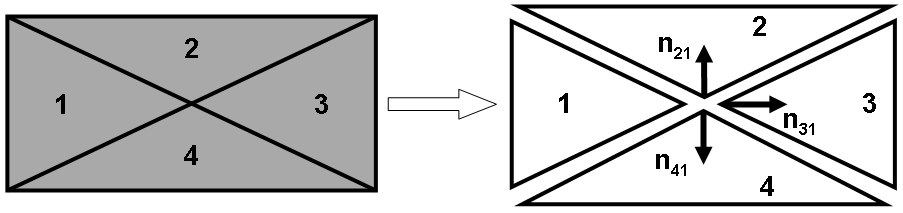
\includegraphics[width=\textwidth]{Contents/Figures/Discontinuities.png}
		\caption{Intersection of four different materials. The interface between different materials is considered as two separated surfaces related by equation \eqref{DobleNodeMatrix}. The vectors $\mathbf{n}_{21}$, $\mathbf{n}_{31}$ and $\mathbf{n}_{41}$ are the unit normal to the surfaces limiting the volume of materials 2, 3, and 4, respectively. In the intersection, equation \eqref{DobleNodeMatrix} is applied to the pairs 2-1, 3-1, and 4-1.}\label{MetodoMultiNodo}
	\end{center}
\end{figure}

\subsection{Field singularities}\label{Singularities}

In the reference \cite{BC-OJOOut} is shown that solving analytically \eqref{RegularizedWeak} is completely equivalent to solve analytically \eqref{CurlCurlWeak}. However, an unexpected problem appears when solving numerically \eqref{RegularizedWeak} with nodal finite elements. As mentioned in \ref{FEMIntro}, a non-physical solution can be obtained when the electromagnetic field is singular on the problem domain. To understand the root causes of this singularity problem, assume that $\mathbf{V}_{h}$ is the vectorial space spanned by $K$ nodal basis functions $N_{i}(\mathbf{r})$ as
\[
\mathbf{V}_{h}:=\left\{\,\mathbf{u}_{h}\,|\,\mathbf{u}_{h} =
\mathbf{\hat{x}}\sum^{K}_{i=1} c_{x_{i}}N_{i}(\mathbf{r}) +
\mathbf{\hat{y}}\sum^{K}_{i=1} c_{y_{i}}N_{i}(\mathbf{r}) +
\mathbf{\hat{z}}\sum^{K}_{i=1} c_{z_{i}}N_{i}(\mathbf{r})\, ,\, 
c_{i} \in \mathbb{C}\,\right\}
\]
with $\mathbf{\hat{n}}\times\mathbf{u}_{h} = 0$ on the PEC surfaces, and
\[
\mathbf{H}^{1}_{0}(\Omega):=\left\{\,\mathbf{F}\in \mathbf{L}^{2}(\Omega)\,\,\,|\,\,\,
\frac{\partial\mathbf{F}}{\partial x},\,
\frac{\partial\mathbf{F}}{\partial y},\,
\frac{\partial\mathbf{F}}{\partial z} \in 
\mathbf{L}^{2}(\Omega)\, , \,\,\mathbf{\hat{n}}\times\mathbf{F} = 0\enspace\text{in PEC}\,\right\}.
\]
It is clear that $\mathbf{V}_{h}$ is included in $\mathbf{H}^{1}_{0}(\Omega)$. But, for non-convex polyhedral
domains, $\mathbf{H}^{1}_{0}(\Omega)$ is strictly included in $\mathbf{H}_{0}(\mathbf{curl},\text{div};\Omega)$ and, moreover, $\mathbf{H}^{1}_{0}(\Omega)$ is closed in $\mathbf{H}_{0}(\mathbf{curl},\text{div};\Omega)$
\cite{CostabelH1CloseH, WeightedRegularizedME}. As a consequence, if \textbf{E}, the analytical solution of \eqref{RegularizedWeak}, belongs to $\mathbf{H}_{0}(\mathbf{curl},\text{div};\Omega)$ but not to $\mathbf{H}^{1}_{0}(\Omega)$; then, it is impossible to approximate \textbf{E} using nodal elements. In fact, such an approximation is impossible using any $\mathbf{H}^{1}$-conforming finite element discretization \cite{CostabelH1Impossible}. This situation happens, for instance, when the electric field is
singular at the corners or edges of a PEC. In other words, for non-convex polyhedral domains,
\[
\mathbf{V}_{h}\subseteq\mathbf{H}^{1}_{0}(\Omega)
\subset\mathbf{H}_{0}(\mathbf{curl},\text{div};\Omega).
\]
If the electric field is singular at some point of the domain, the analytical solution \textbf{E} belongs to
$\mathbf{H}_{0}(\mathbf{curl},\text{div};\Omega)$ but not to $\mathbf{H}^{1}_{0}(\Omega)$. This means that \textbf{E} can not be approximated with nodal elements and \eqref{RegularizedWeak}, because any approximation of \textbf{E}, regardless of the element size or the polynomial order used in the discretization, will belong to $\mathbf{H}^{1}_{0}(\Omega)$. In fact, what is approximated using \eqref{RegularizedWeak} and nodal elements is the Garlekin projection of \textbf{E} onto $\mathbf{H}^{1}_{0}(\Omega)$, which is, in general, globally
different to the physical solution \textbf{E}. An example of this behaviour is shown in Figure \ref{Reg-vs-Ref}.

\begin{figure}[h!]
	\begin{center}
		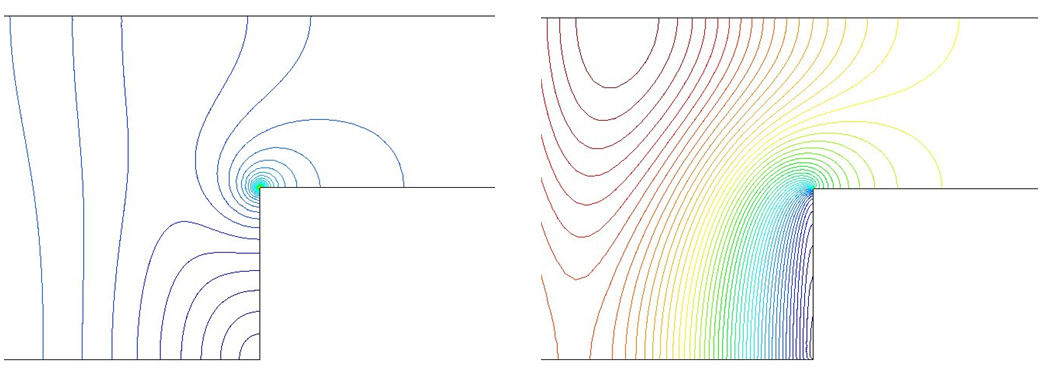
\includegraphics[width=\textwidth]{Contents/Figures/SingularE.png}
		\caption{Modulus of the electric field in a step discontinuity. Left: reference solution. Right: same problem solved with the regularized formulation.}\label{Reg-vs-Ref}
	\end{center}
\end{figure}

A possible solution to the singularity problem is the \textit{Weighted Regularized Maxwell's Equations} (WRME) method explained in \cite{WeightedRegularizedME}. There are other possibilities, such as \cite{SingularFieldMethod, SingularComplementMethod, MixedEdgeNodalFormulation}, but the WRME method is more general and robust. In the WRME method, the divergence term of \eqref{RegularizedWeak} is multiplied by a geometry-dependent weight. This weight tends to zero when approaching to a field singularity. To be more specific, the weight $\alpha$ is
\begin{equation}\label{WRMEWeight}
	\alpha := \left(\,\,\prod_{corners} r^{\gamma_{c}}\,\,\right)\cdot\left(\,\,\prod_{edges} \rho^{\gamma_{e}}\,\,\right),
\end{equation}
where $r$ and $\rho$ are the distances from a point on the domain to the corner or edge where the field is singular. The coefficients $\gamma_{c}$ and $\gamma_{e}$ only depend on the geometry and they can be calculated theoretically beforehand \cite{WeightedRegularizedME}. The WRME method defines the space
\[
\mathbf{X} :=
\left\{\,\mathbf{u}\in\mathbf{H}_{0}(\mathbf{curl};\Omega)\,\,|\,\,
\alpha(\nabla\cdot\mathbf{u})\in {L}^{2}_{loc}(\Omega)\,\right\},
\]
and solves the following weighted regularized weak form: find $\mathbf{E} \in \mathbf{X}$ such that $\forall\,\mathbf{F} \in \mathbf{X}$ holds
\begin{equation}\label{WeigthedRegularizedWeak}
	\begin{aligned}
		\int_{\Omega}\enspace\frac{1}{\mu}\left(\nabla\times\mathbf{E}\right)\cdot\left(\nabla\times\mathbf{\bar{F}}\right)\, + \,\int_{\Omega}\enspace\frac{\alpha}{\tau\mu}\left(\nabla\cdot\left(\varepsilon\mathbf{E}\right)\right)\left(\nabla\cdot\left(\bar{\varepsilon}\mathbf{\bar{F}}\right)\right) \\
		- \enspace\omega^{2}\int_{\Omega}\varepsilon\mathbf{E}\cdot\mathbf{\bar{F}}\enspace + \enspace\textbf{W.R.B.C.}|_{\partial\Omega}\enspace = \enspace i\omega\int_{\Omega}\mathbf{J}\cdot\mathbf{\bar{F}},
	\end{aligned}
\end{equation}
where $\textbf{W.R.B.C.}|_{\partial\Omega}$ is the term, properly adapted to the weighted regularization, that takes into account the boundary conditions: 
\begin{equation}\label{RBCGeneral-WRWF}
	\textbf{W.R.B.C.}|_{\partial\Omega} = \int_{\partial\Omega}\enspace\frac{1}{\mu}\left(\mathbf{\hat{n}}\times\nabla\times\mathbf{E}\right)\cdot\mathbf{\bar{F}}\, - \,\int_{\partial\Omega}\enspace\frac{\alpha}{\tau\mu}\left(\nabla\cdot\left(\varepsilon\mathbf{E}\right)\right)\left(\mathbf{\hat{n}}\cdot\left(\bar{\varepsilon}\mathbf{\bar{F}}\right)\right).
\end{equation}
In \cite{WeightedRegularizedME}, it is demonstrated that solving \eqref{WeigthedRegularizedWeak} is equivalent to solve the Maxwell's equations and also that $\mathbf{H}^{1}_{0}(\Omega)$ is dense in $\mathbf{X}$. These results imply that nodal elements converge to the right electromagnetic field solution even in the presence of singularities.

The method used in ERMES 20.0 to solve the singularity problem is a simplification of the WRME method. Instead of \eqref{WRMEWeight}, ERMES 20.0 uses a weight which is equal to zero in the elements near a singularity and equal to one in the rest. The same idea was applied in \cite{CeroGaugeInCorners} for eddy current problems with the $\mathbf{T}-\Omega$ formulation and, also, in \cite{CeroDivInCorners} for magnetostatic problems with the potential \textbf{A} formulation. In our experience, to achieve the same level of accuracy, the simplified WRME method used in ERMES 20.0 always needed less mesh elements near the singularity and converged faster than the original WRME \eqref{WRMEWeight}.

ERMES 20.0 control the radius of zero weight near the singularity with the so-called \textit{Ungaged Layers} (ULs). Figure \ref{MeshUL} shows an example of a mesh with 3 ULs. When a problem is said to be solved with 1 UL, it means that only the elements with a node in contact with a singularity have a weight equal to zero. If a problem is said to be solved with 2 ULs, it means that the weight is set to zero in the elements with a node in contact with a singularity and also in the elements that have a node in contact with the elements of the first layer. An equivalent definition is applied for 3 ULs, 4 ULs, and so on. Only the elements inside the ULs have a weight $\alpha = 0$. For the rest, the weight $\alpha = 1$. The ULs must be applied in all the places of the domain where the field is singular. The field singularity locations can be known beforehand by just inspecting the geometry of the problem \cite{VanBladel}. Therefore, ULs must be applied to:
\begin{enumerate}
	\item Re-entrant corners and edges of PECs.
	\item Corners and edges of dielectrics.
	\item Intersection of several dielectrics.
\end{enumerate}
Once these points are located, the number of ULs will depend on the size and order of the mesh elements. As an example, it usually requires 3 ULs to solve a singularity with second order elements. But, if very small elements are used around the singularity then, the number of ULs must be increased. On the other hand, if the element order is increased then, the number of ULs can be reduced. The number of ULs has an impact on the conditioning of the matrix, the more ULs are present, the worst is the conditioning. So the less ULs used, the better. More details about the ULs can be found in reference \cite{EMPaper-Me}. 

\begin{figure}[h!]
	\begin{center}
		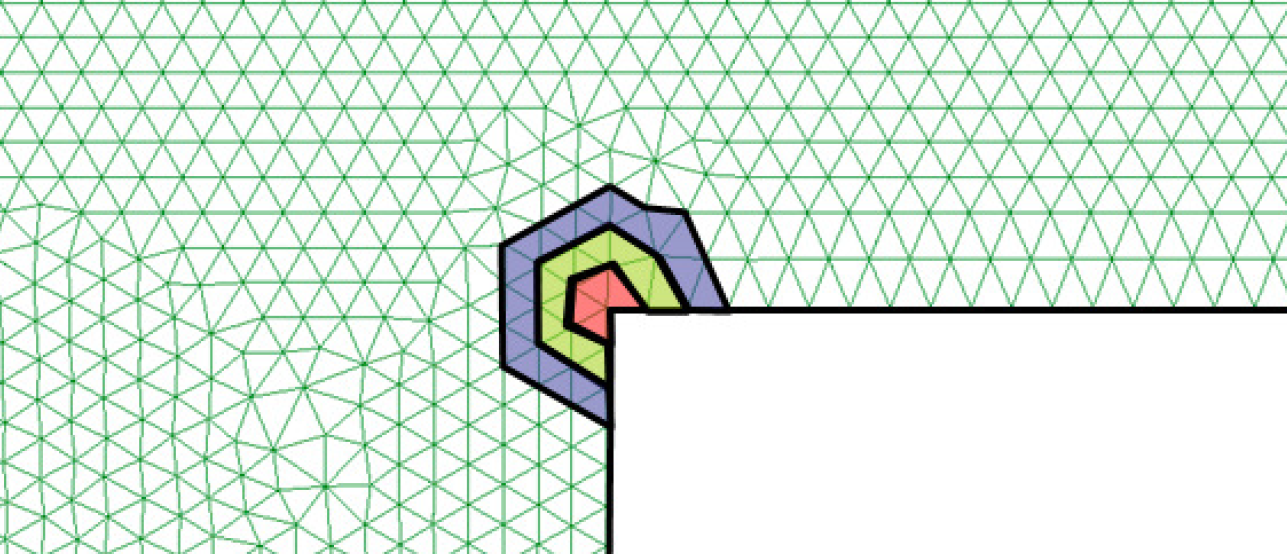
\includegraphics[width=0.9\textwidth]{Contents/Figures/MallaUL.png}
		\caption{Example of a mesh with 3 Ungaged Layers (ULs) around a waveguide edge. In \eqref{WeigthedRegularizedWeak}, the coloured elements will have a weight $\alpha = 0$ and the rest of the elements will have a weight $\alpha = 1$.}\label{MeshUL}
	\end{center}
\end{figure}

\subsection{$\textbf{A}-\phi$ potentials}\label{RMEPotentials}

ERMES 20.0 has available an $\textbf{A}-\phi$ potentials version of the regularized formulation. This version does not provide any additional stability to the nonetheless stable regularized formulation, as is the case with the double-curl formulation \ref{sEdgePotentials}. However, at low frequencies and in the absence of magnetic materials, it allows for solving problems without having to worry about singularities or discontinuities.

The regularized potential version is recommended for problems at low frequencies with non-magnetic materials. At higher frequencies, the singularity problem can re-appear when the skin depth approaches to zero. In the presence of magnetic materials, the normal component of \textbf{A} must be made discontinuous at the interfaces \cite{PotentialsBiro}. ERMES 20.0 solves the singularities and discontinuities of $\textbf{A}-\phi$ with the same techniques as in \ref{Discontinuities} and \ref{Singularities} but adapted to the potentials. The set of differentials equations that the regularized potentials must satisfy is:
\begin{equation}\label{RMAVDE}
	\begin{aligned}
		\nabla\times\left(\frac{1}{\mu}\nabla\times\mathbf{A}\right) - \nabla\left(\frac{1}{\mu}\nabla\cdot\mathbf{A}\right) - \omega^{2}\varepsilon\left(\mathbf{A} + \nabla\phi^{'}\right) &= \mathbf{J},
		\\
		\nabla\left(\omega^{2}\varepsilon\left(\mathbf{A} + \nabla\phi^{'}\right)\right) &= 0,
	\end{aligned}
\end{equation}
where $\phi^{'}$ is defined in \ref{PhiReDef}. On the surface of a perfect electric conductor, the regularized potentials version of the PEC boundary condition is: 
\begin{equation}\label{PEC-AV-RM}
	\begin{aligned}
		\mathbf{\hat{n}}\times\mathbf{A} &= 0,
		\\
		\nabla\cdot\mathbf{A} &= 0,
		\\
		\phi^{'} &= \phi^{'}_{0},
	\end{aligned}
\end{equation}
where $\phi^{'}_{0}$ is the applied voltage defined in equation \ref{PEC-AV-CC}. Similarly, on a PMC symmetry surface, the regularized potentials $\textbf{A}$ and $\phi^{'}$ must satisfy:
\begin{equation}
	\begin{aligned}
		\mathbf{\hat{n}}\times\nabla\times\mathbf{A} &= 0,
		\\
		\mathbf{\hat{n}}\cdot\mathbf{A} &= 0,
		\\
		\mathbf{\hat{n}}\cdot\left(\varepsilon\mathbf{A} + \varepsilon\nabla\phi^{'}\right) &= 0.
	\end{aligned}
\end{equation}
In a Robin boundary surface, where waveguide ports or radiation conditions are applied, the regularized potentials satisfy:
\begin{equation}
	\begin{aligned}
		\mathbf{\hat{n}}\times\nabla\times\mathbf{A} - \gamma(\mathbf{\hat{n}}\times\mathbf{\hat{n}}\times\mathbf{A}) &= \mathbf{U}^{'},
		\\
		\nabla\cdot\mathbf{A} - \gamma\left(\mathbf{\hat{n}}\cdot\mathbf{A}\right) &= \,0,
		\\
		\mathbf{\hat{n}}\cdot\left(\varepsilon\mathbf{A} + \varepsilon\nabla\phi^{'}\right) &= \,0,
	\end{aligned}
\end{equation}
where $\mathbf{U}^{'}$ and $\gamma$ are defined in \ref{RBC-AV-CC}. The above set of equations and boundary conditions are solved in ERMES 20.0 with the following equivalent regularized weak formulation; find an $\mathbf{A} \in \mathbf{H}_{0}(\mathbf{curl};\Omega)$ and $\phi^{'} \in H_{0}(grad;\Omega)$ such
that $\forall\,\mathbf{F} \in \mathbf{H}_{0}(\mathbf{curl};\Omega)$ and $\forall\,G \in H_{0}(grad;\Omega)$ holds:
\begin{equation}\label{Weak-AV-RM}
	\begin{aligned}
		\int_{\Omega}\frac{1}{\mu}(\nabla\times\mathbf{A})\cdot(\nabla\times\mathbf{\bar{F}}) + \int_{\Omega}\frac{1}{\mu}(\nabla\cdot\mathbf{A})(\nabla\cdot\mathbf{\bar{F}})- \omega^{2}\int_{\Omega}\varepsilon\left(\mathbf{A} + \nabla\phi^{'}\right)\cdot\mathbf{\bar{F}}\,&
		\\ 
		+\,\,\textbf{P.R.B.C.}|_{\partial\Omega}\, = \int_{\Omega}\mathbf{J}\cdot\mathbf{\bar{F}},&
		\\
		-\omega^{2}\int_{\Omega}\varepsilon\left(\mathbf{A} + \nabla\phi^{'}\right)\cdot\nabla\bar{G} + \omega^{2}\int_{\partial\Omega}\mathbf{\hat{n}}\cdot\left(\varepsilon\mathbf{A} + \varepsilon\nabla\phi^{'}\right)\bar{G} = 0,&	
	\end{aligned}
\end{equation}
where $\textbf{P.R.B.C.}|_{\partial\Omega}$ accounts for the boundary conditions properly adapted to the regularization and the potentials:
\begin{equation}
	\textbf{P.R.B.C.}|_{\partial\Omega} = \int_{\partial\Omega}\enspace\frac{1}{\mu}\left(\mathbf{\hat{n}}\times\nabla\times\mathbf{A}\right)\cdot\mathbf{\bar{F}}\, - \,\int_{\partial\Omega}\enspace\frac{1}{\mu}(\nabla\cdot\mathbf{A})(\mathbf{\hat{n}}\cdot\mathbf{\bar{F}}).
\end{equation}
In ERMES 20.0, the weak formulation \ref{Weak-AV-RM} has been implemented with first and second order nodal elements for \textbf{A} and first order nodal elements for $\phi^{'}$. 

\section{Local $L^{2}$ projection method with nodal and bubble elements}\label{LL2PNodalBubb}

The Local $L^{2}$ Projection (LL2P) method is a novel approach designed to address the issue with the singularities that affected the regularized formulation (see Section \ref{Singularities}). The LL2P method starts with the regularized weak form \eqref{RegularizedWeak}, using the same parameters and boundary conditions. It then applies local $L^{2}$ projections on the curl and div operators, expanding the unknown fields using first-order nodal basis functions, supplemented by one bubble function within each finite element and three bubble functions on each face of the element \cite{L2P-BE, L2P-BE-P}. Field discontinuities at material interfaces are handled using the procedure described in Section \ref{Discontinuities}; however, singularities require no special treatment. ERMES 20.0 solves the LL2P method with the following weak formulation; if $\mathbf{U}_{h}$ is the space of vectorial functions spanned by first-order nodal finite elements, augmented by one interior bubble within each element and three bubbles functions on each face of each element then, find an $\mathbf{E} \in \mathbf{U}_{h}$ such that $\forall\,\mathbf{F} \in \mathbf{U}_{h}$, the following holds:
\begin{equation}\label{LL2P-Weak}
	\begin{aligned}
		\int_{\Omega}\enspace\frac{1}{\mu}\,\,\mathbf{L}\left(\nabla\times\mathbf{E}\right)\cdot\mathbf{L}\left(\nabla\times\mathbf{\bar{F}}\right)\, + \,\int_{\Omega}\enspace\frac{1}{\tau\mu}\,\,\mathbf{\hat{L}}\left(\nabla\cdot\left(\varepsilon\mathbf{E}\right)\right)\mathbf{\hat{L}}\left(\nabla\cdot\left(\bar{\varepsilon}\mathbf{\bar{F}}\right)\right)
		\\
		\,\,\,\,-\enspace\omega^{2}\int_{\Omega}\varepsilon\mathbf{E}\cdot\mathbf{\bar{F}}\enspace + \enspace \textbf{R.B.C.}|_{\partial\Omega}\enspace = \enspace i\omega\int_{\Omega}\mathbf{J}\cdot\mathbf{\bar{F}},
	\end{aligned}
\end{equation}
where $\mathbf{L}$ and $\mathbf{\hat{L}}$ are local $L^{2}$ projector operators and the rest of the parameters and symbols are described in Section \ref{RMENodal}. The projector operators $\mathbf{L}$ and $\mathbf{\hat{L}}$ are defined as; if $\mathbf{V}_{h}$ is the space of vectorial functions spanned by first order nodal elements and $V_{h}$ is the space of scalar functions spanned by first order nodal elements then, for any $\mathbf{F} \in \mathbf{U}_{h}$ and $\forall\,\mathbf{Q} \in \mathbf{V}_{h}$ and $\forall\,Q \in {V}_{h}$ follows:
\begin{equation}
	\begin{aligned}
	    \int_{\Omega}\,\mathbf{L}\left(\nabla\times\mathbf{F}\right)\cdot\,\mathbf{Q}\, &= \,\int_{\Omega}\,\left(\nabla\times\mathbf{F}\right)\cdot\,\mathbf{Q}\,\, - \, \,\int_{PEC}\,(\mathbf{\hat{n}}\times\mathbf{F})\cdot\mathbf{Q}, 
	    \\
	    \int_{\Omega}\,\mathbf{\hat{L}}\left(\nabla\cdot\left(\varepsilon\mathbf{F}\right)\right) Q\, &= \,\int_{\Omega}\,\left(\nabla\cdot\left(\varepsilon\mathbf{F}\right)\right) Q,	
    \end{aligned}
\end{equation}
Reference \cite{L2P-BE-P} explains in detail how to calculate the FEM matrices from the above expressions. The LL2P weak formulation \eqref{LL2P-Weak} implemented in ERMES 20.0 is a refinement of several options proposed in \cite{L2P-BE, L2P-BE-P} and references therein. This version of the LL2P formulation was selected after extensive testing across a wide range of frequencies and problem types.

\subsection{$\textbf{A}-\phi$ potentials}\label{LL2PPotentials}

ERMES 20.0 also features an $\textbf{A}-\phi$ potentials version of the LL2P formulation. The advantage of this version is that it does not require any special treatment at material interfaces. Following a procedure similar to that of the LL2P \textbf{E}-field version, the next weak form is obtained; find an $\mathbf{A} \in \mathbf{U}_{h}$ and $\phi^{'} \in H_{0}(grad;\Omega)$ such that $\forall\,\mathbf{F} \in \mathbf{U}_{h}$ and $\forall\,G \in H_{0}(grad;\Omega)$ holds:
\begin{equation}\label{LL2P-Weak-AV}
	\begin{aligned}
		\int_{\Omega}\frac{1}{\mu}\,\mathbf{L}\left(\nabla\times\mathbf{A}\right)\cdot\mathbf{L}\left(\nabla\times\mathbf{\bar{F}}\right) + \int_{\Omega}\frac{1}{\mu}\,\mathbf{\hat{L}}\left(\nabla\cdot\mathbf{A}\right)\mathbf{\hat{L}}\left(\nabla\cdot\mathbf{\bar{F}}\right)- \omega^{2}\int_{\Omega}\varepsilon\left(\mathbf{A} + \nabla\phi^{'}\right)\cdot\mathbf{\bar{F}}\,\,&
		\\ 
		+\,\,\textbf{P.R.B.C.}|_{\partial\Omega}\, = \int_{\Omega}\mathbf{J}\cdot\mathbf{\bar{F}},\,&
		\\
		-\omega^{2}\int_{\Omega}\varepsilon\left(\mathbf{A} + \nabla\phi^{'}\right)\cdot\nabla\bar{G} + \omega^{2}\int_{\partial\Omega}\mathbf{\hat{n}}\cdot\left(\varepsilon\mathbf{A} + \varepsilon\nabla\phi^{'}\right)\bar{G} = 0,\,&	
	\end{aligned}
\end{equation}
where all the parameters and symbols have been defined in the previous sections. In ERMES 20.0, the weak formulation \ref{LL2P-Weak-AV} has been implemented with first-order nodal basis functions, plus one bubble function inside each finite element and three bubble functions on each face of each element for \textbf{A} and first order nodal elements for $\phi^{'}$.  

\subsection{Stabilization}\label{LL2PStab}

Reference \cite{L2P-BE} adds a mesh dependant extra stabilization term to the weak forms \ref{LL2P-Weak} and \ref{LL2P-Weak-AV}: 
\begin{equation}
	\begin{aligned}
		\mathbf{S}_{\mathbf{E}} &= h^{2}_{k}\int_{\Omega}\left(\nabla\times\mathbf{E}\right)\cdot\left(\nabla\times\mathbf{\bar{F}}\right)\, + \,h^{2}_{k}\int_{\Omega}\left(\nabla\cdot\mathbf{E}\right) \left(\nabla\cdot\mathbf{\bar{F}}\right),
		\\
		\mathbf{S}_{\mathbf{A}} &= h^{2}_{k}\int_{\Omega}\left(\nabla\times\mathbf{A}\right)\cdot\left(\nabla\times\mathbf{\bar{F}}\right)\, + \,h^{2}_{k}\int_{\Omega}\left(\nabla\cdot\mathbf{A}\right)\left(\nabla\cdot\mathbf{\bar{F}}\right),
	\end{aligned}
\end{equation}
where $h_{k}$ is the element radius. These terms are generally negligible compared to the other terms in \ref{LL2P-Weak} and \ref{LL2P-Weak-AV}. In our experience, they have proven useful only at low frequencies and with a fixed $h_{k} = 1.0$. 








